
\chapter{Einleitung}
\doublespacing
\section{Vorwort}
Dieser Bericht handelt von den Tätigkeiten während der Praxisphase vom 18.10.2021
bis zum 10.01.2022 in der Abteilung Distance & Ranging BU83 bei der
SICK AG in Waldkirch. Ziel war die Fortentwichlung und Neugestaltung der Software des LMS4000 Demokoffers.



\section{Einleitung}
Der LMS4000 ist ein 2D-LiDAR(Light Detection and Ranging)-Sensor der es ermöglicht präzise Vermessungen schnell bewegender, kleiner und großer Objekte unabhängig von ihrer, Farbe oder Oberflächenbeschaffenheit.

Dieser LiDAR-Sensor wird mithilfe des Demokoffers für den Vertrieb demonstriert. Der Koffer beinhaltet mit dem LMS4000 noch drei weitere Sensoren. Zwei von diesen Sensoren sind Metallsensoren, sogenannte Inits, sie werden dazu verwendet, die genaue Winkelposition des LMS4000 zu bestimmen. Der letzte Sensor ist ein Encoder, dieser bestimmt die Veränderung der Position des LMS4000. Mit diesen drei Sensoren kann die Winkelposition des LMS4000 bestimmt werden. Eine SIM1000 wird dazu genutzt, die Daten, die die vier Sensoren liefern, zu erfassen, auszuwerten und zu archivieren (Beschreibung des Demokoffers erweitern).

Mit dem Programm AppStudio ist es möglich, eine App für die SIM1000 zu schreiben. Diese App weist jedem 2D-Scan des LMS4000 eine Winkelposition zu. Somit macht die App es möglich 3D-Bilder mit 60Hz von den möglichen 600Hz des LMS4000 aufzunehmen für 10 Sekunden. Die Bildrate schöpft das Potenzial des LMS4000 nicht aus.

(Um den LMS4000 besser im Vertrieb zu präsentieren wäre es günstig die Bildrate zu erhöhen). Um die Bildrate des Demokoffers zu erhöhen, sollen zwei Apps zusammen arbeiten. Der ScanDriver der von Chris Jorna und die Demokoffer App von Manuel Würzburger..\cite{Ansmann.op.1997,Basler.2016,Fujii.2005,Ierusalimschy.op.2016,Ierusalimschy.2006,Jung.2007,Kuhnel.2012,.,Martin.2013,Young.2014}

\newpage

\section{SICK AG}
\subsection{Geschichte}
Bereits 1946 wurde die heutige SICK AG von Erwin Sick in München gegründet. 1952 hatte
das Unternehmen dann seinen ersten wirtschaftlichen Durchbruch mit der Vorstellung eines
Unfallschutz-Lichtvorhangs auf der Internationalen Werkzeugmesse in Hannover. Der Erfolg
stellte sich ein und die SICK AG ist heute einer der führenden Herstellern und Entwickler
von Sensoren und Sensorlösungen für die Bereiche Fabrik-, Logistik- und Prozessautomation.
1956 zieht das damals 25 Mitarbeiter zählende Unternehmen von München an den heutigen
Standort Waldkirch. Im Jahre 1988 verstirbt Erwin Sick und seine Frau Gisela Sick führt das
Unternehmen als Hauptgesellschafterin fort. 1996 wird eine Umfirmierung des Unternehmens
von der Erwin Sick GmbH in eine Aktiengesellschaft durchgeführt. Der Hauptteil der Aktien
(95%) ist weiterhin in Familienbesitz. Die Restlichen 5% sind Mitarbeiteranteile. Somit ist das
Unternehmen nicht Börsen notiert und kann weiterhin nach Vorstellungen der Gründerfamilie
geführt werden mit nachhaltiger Wachstums Orientierung. Heute umfasst die SICK AG über 50
Tochtergesellschaften und Beteiligungen sowie zahlreiche Vertretungen rund um den Globus. Im
Geschäftsjahr 2021 erzielte das Unternehmen einen Umsatz von 1.964 Millionen Euro
und zählt Weltweit über 10.000 Mitarbeiter.

\begin{figure}[h]
\centering
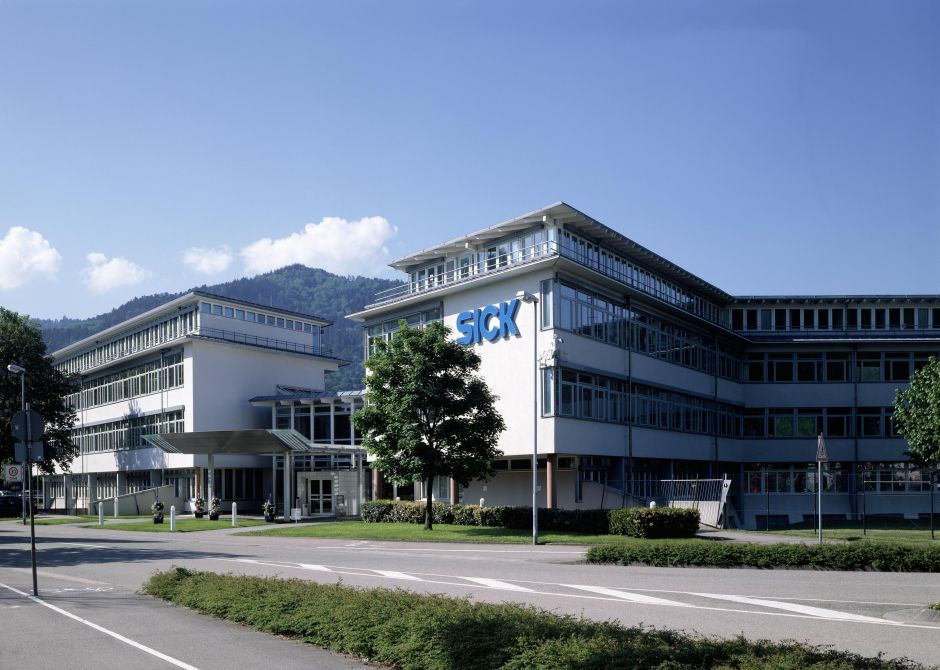
\includegraphics[width=13cm]{Bilder/SICK AG Hauptsitz.jpg}
\caption{Hauptstandort der SICK AG in Waldkirch}
\label{SICK_AG_Hauptsitz}
\end{figure}


\subsection{Unternehmensstruktur}
Wie jedes größere Unternehmen ist auch die SICK AG in verschiedene Bereiche eingeteilt. 
Neben einigen Zentralbereichen, Corporate Departments (CDs) und Corporate Units (CUs), 
gibt es neun unterschiedliche Global Business Centers (GBCs). Jedes GBC hat eine weltweite 
Geschäftsverantwortung für einen bestimmten Technologiebereich. Hier liegt ebenso die 
Verantwortung für die Entwicklung, Produktion und das Produktmanagement von Produkten 
und Serviceleistungen.
Für jede Region gibt es eine zuständige Stelle, welche die Verantwortung für den Vertrieb und 
das Servicegeschäft übernimmt. Dieser Bereich ist in den Sales and Service Clusters (SSCs)
zusammengefasst.
Neben diesen Bereichen gibt es noch Global Intustry Centers (GICs), welche unter anderem 
die Verantwortung für das International Key Account Management (IKAM) und für Branchen 
in der Fabrik-, Logistik- und Prozessautomation innehaben. (SICK AG 2020d)
Die GBCs sind weiterhin in kleinere Einheiten, den sogenannten Business Units (BUs) 
aufgeteilt. Hier wird das Geschäftsfeld der GBC in verschiedene Produkt- und 
Dienstleistungskategorien unterteilt.
Je nach Größe und Ausrichtung einer BU, kann es vorkommen, dass eine weitere Unterteilung 
erfolgt. Hier wird Beispielsweise in Fachdisziplinen wie Entwicklung und Marketing 
aufgeschlüsselt.


\section{Ausgangssituation}

Die Hardware, mit der in diesem Projekt gearbeitet wird, ist der Demokoffer des LMS4000. Dieser wird im Vertrieb genutzt, um die Funktionen des LMS4000 zu demonstrieren. Auf dem Demokoffer lief bis vor kurzem die App von Silas Geschwender. Diese App nutzt nicht das volle Potenzial des LMS4000. Weshalb Manuel Würzburger mithilfe des ScanDrivers von Chris Jona das Potenzial des LMS4000 auszureisen. Der Ersteller hat an dieser neuen App weitergearbeitet, um sie fertig zustellen.

\begin{figure}[h!]
\centering
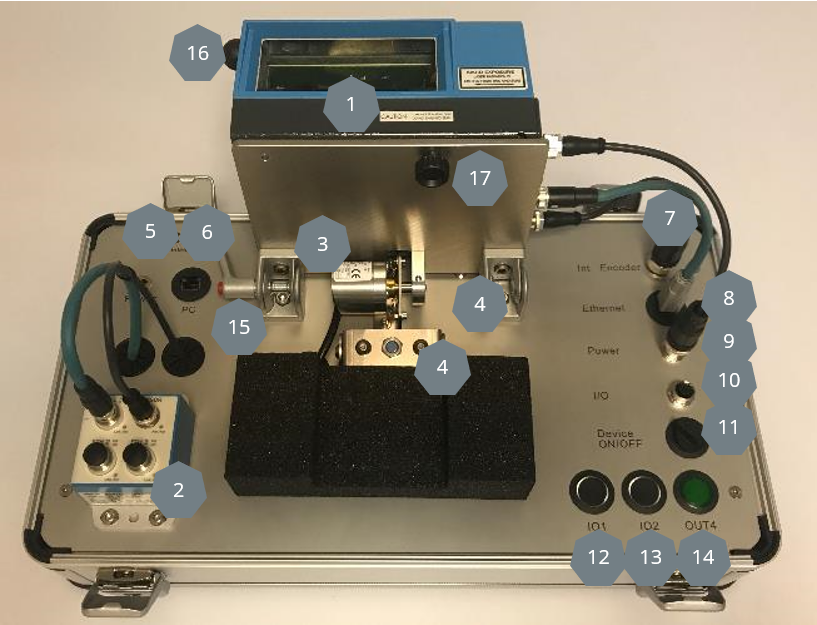
\includegraphics[width=13cm]{Bilder/Demokoffer.png}
\caption{Demokoffer}
\label{Demokoffer}
\end{figure}


\begin{table}[h!]

\begin{tabular}{ll}
1  & LM4111                                \\
2  & SIM1004                               \\
3  & Incremental Encoder                   \\
4  & Inductive Proximity Sensors           \\
5  & Power supply DC 24V                   \\
6  & Ethernet PC                           \\
7  & Internal Encoder                      \\
8  & Ethernet LMS4111                      \\
9  & Power supply LMS4111                  \\
10 & I/Os LMS4111                          \\
11 & Switch ON / OFF LMS4111               \\
12 & IO1 LMS4111                           \\
13 & IO2 LMS4111                           \\
14 & OUT4 LMS4111                          \\
15 & Locking lever for different positions \\
16 & Grab handle                          
\end{tabular}
\caption{Legende zur Abbildung 1.2}
\label{Legende zur Abbildung 12}
\end{table}

An dem Koffer sind vier Sensoren, zwei Metall Sensoren, die, die genau Gradzahl des LMS4000 bestimmen, einmal 0° und um die 90° Position zu bestimmen. Der Encoder kann Rotation feststellen und damit die Veränderung der Gradzahl.
Der LMS4000 nimmt ein 2D-Bild auf, welches einer Gradzahl zugewiesen wird. Die SIM1004 verarbeitet diese Daten zu einer Punktewolke.

\section{Aufgabenstellung}
Das Hauptziel ist es, die App auf eine stabile Version für den Vertrieb zu bringen. Fehler und Störungen sollen korrigiert werden. Ein weiteres Ziel ist es zu erforschen, welche die höchst mögliche Frequenzzahl ist, mit welcher aufgenommen werden kann. Die ursprüngliche App von Silas Geschwender konnte mit 60Hz für 10 Sekunden aufnehmen. Es muss bestimmt werden, mit welcher Herzfrequenz aufgenommen werden kann und die SIM noch stabil läuft. Auch soll das Design der App maßgeblich verändert werden. Die App besteht aus zwei Seiten, auf der ersten Seite stehen die Daten der Komponenten, Status des Demokoffers und hier können auch neue Scans aufgenommen werden. Der aktuelle Scann ist dort auch zu sehen, die älteren Scans sind auch der zweiten Seite zu sehen, wo sie auch heruntergeladen oder gespeichert werden können. Die Seite zum Aufnehmen der Scans und die Seite zum Einsehen der Scans sollen zusammengefasst werden.
